\begin{figure}[htbp]
			\centering
			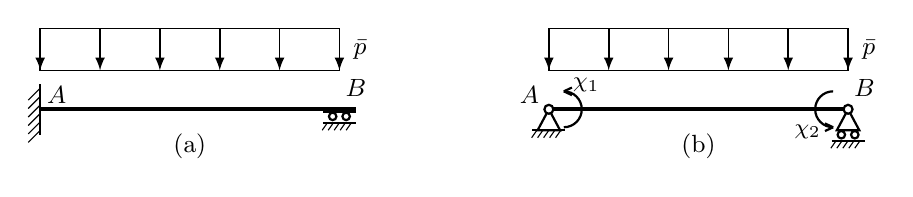
\begin{tikzpicture}[scale=0.95,>=latex,
				trave/.style={line width=1.4pt},
				carico/.style={black, line width=0.6pt},
				forza/.style={black, line width=0.8pt},
				]
				% ── Parametri ──
				\def\tw{0.15}\def\thR{0.28}\def\rn{0.06}
				\def\rw{0.05}\def\bw{0.09}\def\gw{0.22}\def\hh{0.10}
				\def\twall{0.16}\def\hwall{0.34}
				\def\Lell{4}\pgfmathsetmacro{\xMid}{0.5*\Lell}
				\def\pBot{0.52}\def\pTop{1.08}                 % riquadro del carico (chiusura sulle punte = \pBot)
				\def\rCoppia{0.24}\def\Lwing{0.12}\def\AoffX{0.20}\def\BoffX{0.20}
				% ── Vincoli ──
				\def\incastro#1{%
					\draw[thick] (#1,-\hwall) -- (#1,\hwall);
					\foreach \i in {-2.5,-1.5,-0.5,0.5,1.5,2.5}
					\draw[thin] (#1,{\i*\hwall/3}) -- ++(-\twall,-\twall);}
				\def\cerniera#1{%
					\draw[thick] (#1,0) -- (#1-\tw,-\thR) -- (#1+\tw,-\thR) -- cycle;
					\draw[thick] (#1-\gw,-\thR) -- (#1+\gw,-\thR);
					\foreach \x in {-0.16,-0.08,0,0.08,0.16}\draw[thin] (#1+\x,-\thR) -- ++(-0.07,-\hh);
					\draw[thick, fill=white] (#1,0) circle (\rn);}
				\def\carrello#1{%
					\draw[thick] (#1,0) -- (#1-\tw,-\thR) -- (#1+\tw,-\thR) -- cycle;
					\draw[thick] (#1-\bw,-\thR-\rw-0.01) circle (\rw);
					\draw[thick] (#1+\bw,-\thR-\rw-0.01) circle (\rw);
					\draw[thick] (#1-\gw,-\thR-2*\rw-0.04) -- (#1+\gw,-\thR-2*\rw-0.04);
					\foreach \x in {-0.16,-0.08,0,0.08,0.16}\draw[thin] (#1+\x,-\thR-2*\rw-0.04) -- ++(-0.07,-\hh);
					\draw[thick, fill=white] (#1,0) circle (\rn);}
				% ── Glifo: piatto rigido (no perno) + ruote + barra di terra (scorrimento orizzontale) ──
				\def\glifo#1{%
					\draw[thick] (#1-\gw,-0.03) -- (#1+\gw,-0.03);
					\draw[thick] (#1-\bw,-0.03-\rw-0.015) circle (\rw);
					\draw[thick] (#1+\bw,-0.03-\rw-0.015) circle (\rw);
					\draw[thick] (#1-\gw,-0.03-2*\rw-0.05) -- (#1+\gw,-0.03-2*\rw-0.05);
					\foreach \x in {-0.16,-0.08,0,0.08,0.16}\draw[thin] (#1+\x,-0.03-2*\rw-0.05) -- ++(-0.07,-\hh);}
				% ── Carico uniforme: riquadro chiuso (chiusura inferiore sulle punte), fino all'incastro ──
				\def\caricodist{%
					\draw[carico] (0,\pBot) rectangle (\Lell,\pTop);
					\foreach \x in {0,0.8,1.6,2.4,3.2,4.0}\draw[->, carico] (\x,\pTop) -- (\x,\pBot);
					\node[right, font=\small] at (\Lell+0.06,{0.5*(\pBot+\pTop)}) {$\bar{p}$};}
				% ── Coppie antiorarie che attraversano la trave (come mu_A, mu_B del template) ──
				\def\coppiaA#1{%
					\draw[forza] (\AoffX,-\rCoppia) arc[start angle=-90, end angle=90, radius=\rCoppia];
					\draw[forza] (\AoffX,\rCoppia) -- ({\AoffX+\Lwing*cos(25)},{\rCoppia+\Lwing*sin(25)});
					\draw[forza] (\AoffX,\rCoppia) -- ({\AoffX+\Lwing*cos(-25)},{\rCoppia+\Lwing*sin(-25)});
					\node[font=\footnotesize] at (\AoffX+0.3,\rCoppia+0.08) {#1};}
				\def\coppiaB#1{%
					\draw[forza] (\Lell-\BoffX,\rCoppia) arc[start angle=90, end angle=270, radius=\rCoppia];
					\draw[forza] (\Lell-\BoffX,-\rCoppia) -- ({\Lell-\BoffX+\Lwing*cos(155)},{-\rCoppia+\Lwing*sin(155)});
					\draw[forza] (\Lell-\BoffX,-\rCoppia) -- ({\Lell-\BoffX+\Lwing*cos(205)},{-\rCoppia+\Lwing*sin(205)});
					\node[font=\footnotesize] at (\Lell-\BoffX-\rCoppia-0.1,-0.30) {#1};}
				
				% ===================== (a) schema iniziale: incastro + glifo =====================
				\begin{scope}[xshift=0cm]
					\draw[trave] (0,0) -- (\Lell+\gw,0);     % trave estesa fino al bordo del piatto del glifo
					\incastro{0}\glifo{\Lell}
					\caricodist
					\node[above, font=\small] at (0.22,-0.05) {$A$};
					\node[above, font=\small] at (\Lell+\gw,0.04) {$B$};
					\node[font=\small] at (\xMid,-0.50) {(a)};
				\end{scope}
				
				% ===================== (b) sistema principale: cerniera + carrello + coppie =====================
				\begin{scope}[xshift=6.8cm]
					\draw[trave] (0,0) -- (\Lell,0);
					\cerniera{0}\carrello{\Lell}
					\caricodist
					\coppiaA{$\chi_1$}
					\coppiaB{$\chi_2$}
					\node[above left, font=\small] at (-0.,-0.05) {$A$};
					\node[above, font=\small] at (\Lell+\gw,0.04) {$B$};
					\node[font=\small] at (\xMid,-0.50) {(b)};
				\end{scope}
				
			\end{tikzpicture}
			\caption{Trave con incastro e glifo (a) e sistema principale scelto (b).}
			\label{fig:stat_iper_trasv_01}
		\end{figure}
